%%%%%%%%%%%%%%%%%%%%%%
%%Options for presentations (in-class) and handouts (e.g. print). 
\documentclass[pdf
%,handout
]{beamer}
\usepackage{pgfpages}
%\pgfpagesuselayout{2 on 1}[letterpaper,border shrink=5mm]

\graphicspath{{../}}
%%%%%%%%%%%%%%%%%%%%%%
%% Change this for different slides so it appears in bar
\usepackage{authoraftertitle}
\date{6.2: Complex Numbers; Polar Form}

%%%%%%%%%%%%%%%%%%%%%%
%% Upload common style file
\usepackage{../LyryxLinearAlgebraSlidesStyle}

\begin{document}
	
	%%%%%%%%%%%%%%%%%%%%%%%
	%% Title Page and Copyright Common to All Slides	
	%Title Page
	\input ../frontmatter/titlepage.tex	
	%LOTS Page
	%\input frontmatter/lyryxopentexts.tex	
	%Copyright Page
	\input ../frontmatter/copyright.tex	
	%%%%%%%%%%%%%%%%%%%%%%%%%

\section{Polar Form}
%-------------- start slide -------------------------------%
\frame{\frametitle{Complex Numbers in Polar Form}
Suppose $z=a+bi$, and let $\textcolor{blue}{r}=|z|=\sqrt{a^2+b^2}$.  
Then $\textcolor{blue}{r}$ is the distance from $z$ to the origin.
Denote by $\alert{\theta}$ the angle that the line through $0$ and $z$
makes with the positive $x$-axis (measured clockwise).

\begin{picture}(3,1.75)
\put(1.25,0){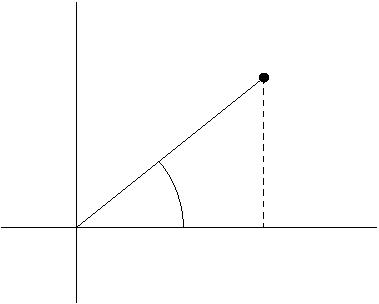
\includegraphics[scale=.75]{figures/polar.pdf}}
{\small
\put(1.5,0.25){$0$}
\put(2.9,0.25){$x$}
\put(1.5,1.3){$y$}
\put(2.65,1.1){$z=a+bi$}
\put(2.15,0.25){$a$}
\put(2.6,0.7){$b$}
\put(2.05,0.8){$\textcolor{blue}{r}$}
\put(1.85,0.43){$\alert{\theta}$}
}
\end{picture}

\pause
Then $\theta$ is an angle defined by
$\cos\theta = \frac{a}{r}$ and $\sin\theta=\frac{b}{r}$, so

\vspace*{-.15in}
\[ z=r\cos\theta +r\sin\theta i=r(\cos\theta + i\sin\theta).\] 

\pause
$\theta$ is called \alert{an argument of $z$}, and is
denoted $\arg z$.
}
%-------------- end slide -------------------------------%

%-------------- start slide -------------------------------%
\frame{\frametitle{The Polar Form}
\begin{definition}[Polar Form of a Complex Number]
Let $z$ be  a complex number with $|z|=r$ and $\arg z=\theta$. 
Then 
\vspace*{-.1in}

\[ z=re^{i\theta}=r(\cos\theta + i\sin\theta )\]
\vspace*{-.2in}

is called \alert{a polar form} of $z$.
\end{definition}

\pause

Since $\arg z$ is not unique, we do not write \alert{the}
polar form of $z$.

\pause
\begin{definition}
Let $z$ be a complex number with $|z|=r$.
The \alert{principal argument} of $z$
is the unique angle $\theta=\arg z$ (measured in radians) such that 
\vspace*{-.1in}

\[ -\pi < \theta \leq \pi. \]
\end{definition}
}
%-----------------end slide------------------%

%----------------start slide------------------%
\frame{
\begin{example}
Find the polar form for the number $z=1$. 
\end{example}
\pause

\begin{solution}\em 
To convert $z$ to polar form, we need to find $r$ and $\theta$ 
so that $1=re^{i\theta}$.
\pause
Now $r=|z|=\sqrt{1^2}=1$,
\pause
and $\theta=0$ is an argument for $z=1$.
\pause
However, we may also write

\[ 1=e^{2\pi i}, 1=e^{-2\pi i}, e^{4\pi i}, e^{6\pi i}, \ldots \]

\pause
Since sine and cosine have periodicity $2\pi$, we may add (or subtract)
multiples of $2\pi$ to any argument.
\end{solution}
}
%-------------- end slide -------------------------------%

%------------------start slide---------------------------%
\frame{\frametitle{Converting to Polar Form}
\begin{example}
Conver the number $z = -2 +2\sqrt{3}i$ to polar form.
\end{example}
\pause

\begin{solution}\em
To convert $z$ to polar form, 
we need to find $r$ and $\theta$ so that
$-2+2\sqrt{3}i=re^{i\theta}$.
\pause
Since $r=|z|$, 
\[ r=\sqrt{(-2)^2 + (2\sqrt{3})^2}
\pause = \sqrt{4+4(3)}
\pause = \sqrt{16} \pause = 4.\]
\pause
\vspace*{-.25in}

There are two approaches to finding an argument, $\theta$.
\pause
One is to graph $-2+2\sqrt{3}$ in the complex plane.

\begin{picture}(3,0.95)
\put(1.5,0){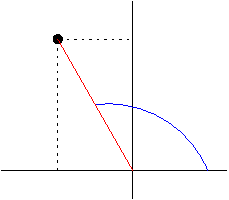
\includegraphics[scale=.75]{figures/polar-2.pdf}}
{\tiny
\put(2.20,0.04){$0$}
\put(2.6,0.04){$x$}
\put(2.05,0.9){$y$}
\put(1.31,0.81){$(-2, 2\sqrt{3})$}}
{\tiny
\put(1.57,0.4){$2\sqrt{3}$}
\put(1.89,0.05){$2$}}
{\scriptsize
\put(1.9,0.38){\alert{$4$}}
\put(2.4,0.4){\textcolor{blue}{$\theta$}}
}
\end{picture}
\end{solution}
}
%----------------end slide-------------------%

%------------start slide---------------------%
\frame{
\begin{solution}[continued]\em
The triangle sitting on the negative half of the real axis
has sides of length $2$, $2\sqrt 3$, and $4$; 
\pause
you should
recognize this as a right triangle whose other two angles
measure $\frac{\pi}{3}$ and $\frac{\pi}{6}$.  
\pause
From this, we see that $\theta=\frac{2\pi}{3}$ is an
argument of $z$.
\pause

\alert{Therefore, $z$ can be written in polar form as $z=4e^{i(2\pi/3)}.$}
\pause
\medskip

The other approach to finding an argument, $\theta$, 
for $z=-2+2\sqrt{3}i$ is as follows. 
We've already calculated $|z|=r=4$.  
By definition, $\theta$ is an angle satisfying
\pause
\[ \cos\theta=\frac{-2}{4} \pause = -\frac{1}{2}
\pause
\mbox{ and }
\sin\theta=\frac{2\sqrt{3}}{4} \pause = \frac{\sqrt{3}}{2}.\]
\pause
By graphing the point $(-\frac{1}{2}, \frac{\sqrt{3}}{2})$, 
we again determine that $\theta=\frac{2\pi}{3}$, and thus
\alert{$z$ can be written in polar form as $z=4e^{i(2\pi/3)}.$}
\end{solution}
}
%----------------------end slide -------------------------%

%-------------- start slide -------------------------------%
\frame{
\begin{block}{Exercises}
Convert each of the following complex numbers to polar form.
\begin{enumerate}
\item $3i$
\pause
\textcolor{blue}{$=3e^{(\pi/2)i}$.}
\pause
\item $-1-i$
\pause
\textcolor{blue}{$=\sqrt{2}e^{-(3\pi/4)i}
\pause =\sqrt{2}e^{(5\pi/4)i}$.}
\pause
\item $\sqrt{3} - i$
\pause
\textcolor{blue}{$=2e^{-(\pi/6)i}$.}
\pause
\item $\sqrt{3}+3i$
\pause
\textcolor{blue}{=$2\sqrt{3}e^{(\pi/3)i}$.}
\end{enumerate}
\end{block}
}
%-------------- end slide -------------------------------%

%------------------start slide-----------------------------%
\frame{\frametitle{Converting from Polar Form to Cartesian form}
\begin{problem}\em
Let $z= 2e^{2\pi i / 3}$. Write $z$ in the form $z=a+bi$
(this is called \alert{Cartesian form} or \alert{Standard form}).
\end{problem}
\pause
\begin{solution}\em
First, remember that $e^{i\theta}=\cos\theta +i\sin\theta$, 
\pause
and thus
\begin{eqnarray*}
e^{2\pi i/3} &=& \cos (2 \pi /3) + i \sin(2\pi/3) \\
\pause
&=& -\frac{1}{2} + i \frac{\sqrt{3}}{2}.
\end{eqnarray*}
\pause
Therefore
\begin{eqnarray*}
z = 2e^{2\pi i/3} \pause
&=& 2 \left( -\frac{1}{2} + i \frac{\sqrt{3}}{3} \right) \\
\pause
&=& -1 + \sqrt{3} i.
\end{eqnarray*}
\end{solution}
}
%-------------- end slide -------------------------------%

%------------------start slide-----------------------------%
\frame{
\begin{block}{Exercises}
Express each of the following complex numbers in Cartesian
form.
\begin{enumerate}
\item $3e^{-\pi i}$
\pause
\textcolor{blue}{$=-3$}
\pause
\item $2e^{3\pi i/4}$
\pause
\textcolor{blue}{$=-\sqrt{2}+i\sqrt{2}$}
\pause
\item $2\sqrt{3}e^{-2\pi i/6}$
\pause
\textcolor{blue}{$=\sqrt{3}-3i$}
\end{enumerate}
\end{block}

}
%------------------------end slide-----------------------%

%-------------- start slide -------------------------------%
{\small
\frame{\frametitle{Using the Polar Form}
Problems involving multiplication of complex numbers can often
be solved more easily by using polar forms of the complex numbers.
\pause
\begin{theorem}\em
If $z_1=r_1e^{i\theta_1}$ and $z_2=r_2e^{i\theta_2}$
are complex numbers, then
\[ z_1z_2=r_1r_2e^{i(\theta_1+\theta_2)}\]
\end{theorem}
\pause

\begin{theorem}[De Moivre's Formula]\em
If $\theta$ is any angle and $n$ is a positive integer, then  $\displaystyle \left( e^{i \theta} \right)^n = e^{i n \theta}.$
Equivalently,  
%%\[ \left( r\left( \cos \theta+i\sin \theta\right) \right)^{n}
%%=r^{n}\left( \cos n \theta +i\sin n\theta\right). \]
\begin{eqnarray*}
	 \left( \cos \theta+i\sin \theta\right) ^{n}&=& \left( \cos n \theta +i\sin
	n\theta\right) 
\end{eqnarray*}
\end{theorem}
\pause
\begin{alertblock}{}
As an immediate consequence of De Moivre's Formula, we have that
for any real number $r>0$ and any positive integer $n$, 
%%\[ \left( r\left( \cos \theta+i\sin \theta\right) \right)^{n}
%%=r^{n}\left( \cos n \theta +i\sin n\theta\right). \]
\begin{eqnarray*}
 (re^{i\theta})^n &=& r^n e^{in\theta} \\
\left( r\left( \cos \theta+i\sin \theta\right) \right) ^{n}&=&r^{n}\left( \cos n \theta +i\sin
n\theta\right) 
\end{eqnarray*}
\end{alertblock}
}}
%-------------- end slide -------------------------------%

%-------------- start slide -------------------------------%
\frame{
\begin{problem}\em
Express $(1-i)^6(\sqrt{3}+i)^3$ in the form $a+bi$.
\end{problem}
\pause
\begin{solution}\em
Let $z=1-i=\sqrt{2}e^{-\pi i/4}$ and
$w=\sqrt{3}+i=2e^{\pi i/6}$.
\pause
We want to compute $z^6w^3$.
\pause
\begin{eqnarray*}
z^6w^3 & = & (\sqrt{2}e^{-\pi i/4})^6(2e^{\pi i/6})^3 \\
\pause
& = & (2^3 e^{-6\pi i/4}) (2^3 e^{3\pi i/6}) \\
\pause
& = & (8 e^{-3\pi i/2}) (8 e^{\pi i/2}) \\
\pause
%& = & 64 e^{(-3\pi/2)i+(\pi/2)i} \\
& = & 64 e^{-\pi i}\\
\pause
& = & 64 e^{\pi i} \\
\pause
& = & 64(\cos\pi + i\sin\pi) \\
\pause
& = & -64. 
\end{eqnarray*}
\end{solution}
}
%-------------- end slide -------------------------------%

%-------------- start slide -------------------------------%
\frame{
\begin{problem}\em
Express $\left(\frac{1}{2}-\frac{\sqrt{3}}{2}i\right)^{17}$ in the form $a+bi$.
\end{problem}
\pause
\begin{solution}\em
Let $z=\frac{1}{2}-\frac{\sqrt{3}}{2}i=e^{-\pi i/3}$.
\pause
Then
\begin{eqnarray*}
z^{17} & = & \left(e^{-\pi i/3}\right)^{17} \\
\pause
& = & e^{-17\pi i/3} \\
\pause
& = & e^{\pi i/3} \\
\pause
& = & \cos\frac{\pi}{3} +i\sin\frac{\pi}{3} \\
\pause
& = & \frac{1}{2}+\frac{\sqrt{3}}{2}i.
\end{eqnarray*}
\end{solution}
}
%-------------- end slide -------------------------------%

\end{document}
